\documentclass[12pt,letterpaper]{exam}
\usepackage[lmargin=1in,rmargin=1in,tmargin=1in,bmargin=1in]{geometry}
\usepackage{../style/exams}

% -------------------
% Course & Exam Information
% -------------------
\newcommand{\course}{MATH 141: Exam 3}
\newcommand{\term}{Spring --- 2025}
\newcommand{\examdate}{04/18/2025}
\newcommand{\timelimit}{50 Minutes}

\setbool{hideans}{false} % Student: True; Instructor: False


% -------------------
% Content
% -------------------
\begin{document}

\examtitle
\instructions{Write your name on the appropriate line on the exam cover sheet. This exam contains \numpages\ pages (including this cover page) and \numquestions\ questions. Check that you have every page of the exam. Answer the questions in the spaces provided on the question sheets. Be sure to answer every part of each question and show all your work. If you run out of room for an answer, continue on the back of the page --- being sure to indicate the problem number.} 
\scores
\bottomline
\newpage

% -------------------
% Questions
% -------------------
\begin{questions}

% Question 1
\newpage
\question[16] Consider the function $f(x)= x(6 - x)$ plotted below.
		\[
            	\fbox{
            	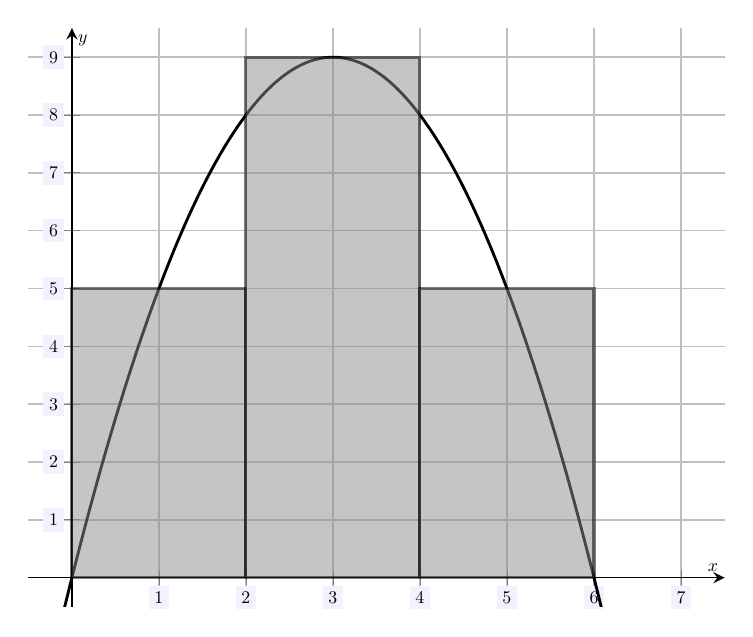
\begin{tikzpicture}[scale=1.29,every node/.style={scale=0.5}]
            	\begin{axis}[
            	grid=both,
            	axis lines=middle,
            	ticklabel style= {fill= blue!5!white},
            	xmin= -0.5, xmax=7.5,
            	ymin= -0.5, ymax=9.5,
            	xtick= {-10,-9,...,10},
            	ytick= {-10,-9,...,10},
            	minor tick = {-10,-9,...,10},
            	xlabel= \(x\), ylabel= \(y\)
            	]
		\addplot[thick, samples=150, smooth, domain= -10.5:10.5] {x*(6 - x)};  
		
		\remove{\draw[line width=0.03cm,fill=gray!90,opacity=0.5] (0,0) -- (2,0) -- (2,5) -- (0,5) -- (0,0);}
		\remove{\draw[line width=0.03cm,fill=gray!90,opacity=0.5] (2,0) -- (4,0) -- (4,9) -- (2,9) -- (2,0);}
		\remove{\draw[line width=0.03cm,fill=gray!90,opacity=0.5] (4,0) -- (6,0) -- (6,5) -- (4,5) -- (4,0);}
            	\end{axis}
            	\end{tikzpicture}
            	}
            	\]

\begin{enumerate}[(a)]
\item Approximate the area under the curve $f(x)$ on $[0, 6]$ with a Riemann sum using a midpoint sum with $n= 3$ boxes---all with equal width. \pspace

\sol{We break the interval $[a, b]= [0, 6]$ into $n= 3$ subintervals (one for each box) and each will have equal width. Therefore, the width of each box is\dots
	\[
	\Delta x= \dfrac{b - a}{n}= \dfrac{6 - 0}{3}= \dfrac{6}{3}= 2
	\]
But then the subintervals are $[0, 2]$, $[2, 4]$, and $[4, 6]$. We are using a midpoint sum, so we use the midpoint of each subinterval as the $x$-value to find the height of each box. These $x$-values are $x= 1$, $x= 3$, and $x= 5$. Observe that\dots
	\[
	\begin{aligned}
	f(1)&= 1(6 - 1)= 1(5)= 5 \\
	f(3)&= 3(6 - 3)= 3(3)= 9 \\
	f(5)&= 5(6 - 5)= 5(1)= 5
	\end{aligned}
	\]
Recall the area of each rectangle is $A= hb= f(x) \Delta$. Therefore, we have\dots
	\[
	\begin{aligned}
	\text{Area under } f(x)&\approx \sum_{i=1}^4 A_i \\
	&= \sum_{i=1}^4 f(x_i) \Delta x \\
	&= f(1) \cdot \Delta x + f(3) \cdot \Delta x + f(5) \cdot \Delta x \\
	&= 5(2) + 9(2) + 5(2) \\
	&= 10 + 18 + 10 \\
	&= 38
	\end{aligned}
	\]
}

\item Sketch this approximation on the graph given above. 
\end{enumerate}



% Question 2
\newpage
\question[14] Showing all your work and simplifying your result, compute the following:
	\[
	\dfrac{d}{dx} \int_{e^x}^8 \dfrac{\sin t}{t} \;dt
	\] \pspace

\sol{Using the Fundamental Theorem of Calculus, we know\dots
	\[
	\dfrac{d}{dx} \int_{e^x}^8 \dfrac{\sin t}{t} \;dt= \dfrac{d}{dx} -\int_8^{e^x} \dfrac{\sin t}{t} \;dt= -\dfrac{\sin(e^x)}{e^x} \cdot \dfrac{d}{dx} \, \left( e^x \right)= -\dfrac{\sin(e^x)}{e^x} \cdot e^x = -\sin(e^x)
	\]
} \vfill \vspace{3cm}



% Question 3
\question[14] Suppose $f(x)$ is a function such that $f(5)= 9$ and $\ds\int_0^5 f'(x) \;dx= 11$. Showing all your work, compute $f(0)$. \pspace

\sol{By the Fundamental Theorem of Calculus, if $F(x)$ is an antiderivative of $f(x)$, then we know that\dots
	\[
	\int_a^b f(x) \;dx= F(b) - F(a)
	\]
Observe that $f(x)$ is an antiderivative for $f'(x)$ because $\dfrac{d}{dx} \, f(x)= f'(x)$. But then\dots	
	\[
	\begin{gathered}
	\int_0^5 f'(x) \;dx= f(5) - f(0) \\[0.3cm]
	11= 9 - f(0) \\[0.3cm]
	f(0)= 9 - 11 \\[0.3cm]
	f(0)= -2
	\end{gathered}
	\]
} \vfill



% Question 4
\newpage
\question[20] Showing all your work, compute the following: \par\vspace{0.3cm}
	\begin{enumerate}[(a)]
	\item $\ds\int \dfrac{3x^5 + 2x^2 - x}{x^3} \;dx$ \vfill
	
	\sol{
		\[
		\int \dfrac{3x^5 + 2x^2 - x}{x^3} \;dx= \int \left(3x^2 + \dfrac{2}{x} - \dfrac{1}{x^2} \right) \;dx= x^3 + 2\ln|x| + \dfrac{1}{x} + C
		\] 
	} \vfill
	
	\item $\ds\int \left( 2^x + \cos x - \tan x \right) \;dx$ \vfill
	
	\sol{
		\[
		\int \left( 2^x + \cos x - \tan x \right) \;dx= \dfrac{2^x}{\ln 2} + \sin x - \ln|\sec x| + C
		\] 
	\pspace
		
	{\scriptsize Note. Using $\int \tan x \;dx= -\ln|\cos x| + C$, one could also answer $\dfrac{2^x}{\ln 2} + \sin x + \ln|\cos x| + C$.} } \vfill
	
	\item $\ds\int_0^1 \left(x - x^{3/2} \right) \;dx$ \vfill
	
	\sol{
		\[
		\int_0^1 \left(x - x^{3/2} \right) \;dx= \dfrac{x^2}{2} - \dfrac{2}{5} \, x^{5/2} \bigg|_{x=0}^{x=1}= \left( \dfrac{1}{2} - \dfrac{2}{5} \right) - \left( 0 - 0 \right)= \dfrac{5}{10} - \dfrac{4}{10}= \dfrac{1}{10}
		\] 
	} \vfill
	\end{enumerate}



% Question 5
\newpage
\question[16] Consider the shaded area shown below.
		\[
            	\fbox{
            	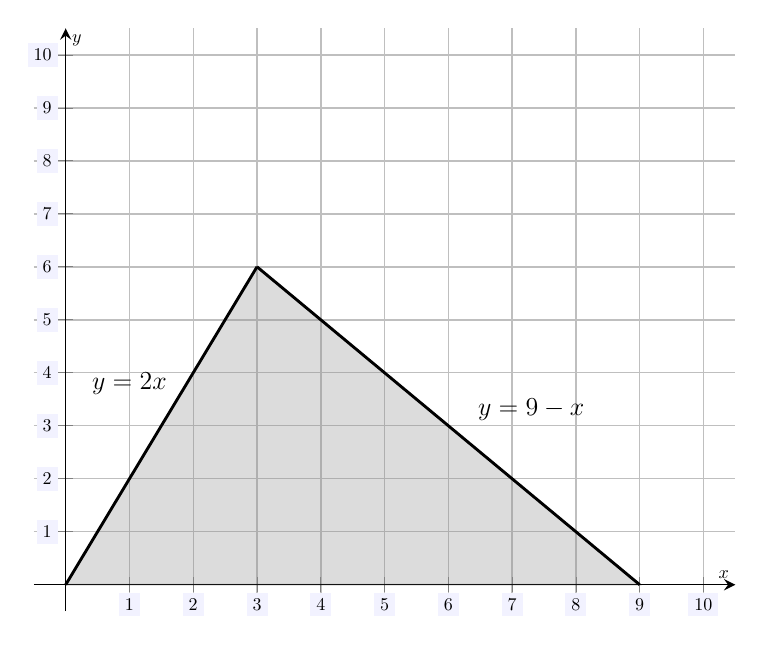
\begin{tikzpicture}[scale=1.3,every node/.style={scale=0.5}]
            	\begin{axis}[
            	grid=both,
            	axis lines=middle,
            	ticklabel style= {fill= blue!5!white},
            	xmin= -0.5, xmax=10.5,
            	ymin= -0.5, ymax=10.5,
            	xtick= {-10,-9,...,10},
            	ytick= {-10,-9,...,10},
            	minor tick = {-10,-9,...,10},
            	xlabel= \(x\), ylabel= \(y\)
            	]
		\draw[fill=gray!90,opacity=0.3] (0,0) -- (3,6) -- (9,0) -- (0,0);
		\node at (1,3.8) {\Large$y= 2x$};
		\addplot[thick, samples=5, smooth, domain= 0:3] {2*x};  
		\node at (7.3,3.3) {\Large$y= 9 - x$};
		\addplot[thick, samples=5, smooth, domain= 3:9] {9 - x};  
            	\end{axis}
            	\end{tikzpicture}
            	}
            	\]

\begin{enumerate}[(a)]
\item Set up \textit{\bfseries but do not evaluate} an integral expression \textit{\bfseries with respect to $x$} which computes the shaded area. \vfill

\sol{
	\[
	\int_0^3 (2x - 0) \;dx + \int_3^9 \big( (9 - x) - 0 \big) \;dx 
	\] 
} \vfill

\item Set up \textit{\bfseries but do not evaluate} an integral expression \textit{\bfseries with respect to $y$} which computes the shaded area. \vfill

\sol{
	\[
	\int_0^6 \bigg( (9 - y) - \dfrac{y}{2} \bigg) \;dy
	\]
} \vfill
\end{enumerate}



% Question 6
\newpage
\question[20] Showing all your work, compute the following: \par\vspace{0.3cm}
	\begin{enumerate}[(a)]
	\item $\ds\int \dfrac{x}{x + 3} \;dx$ \pspace
	
	\sol{Let $u= x + 3$, so that $x= u - 3$. Then $du= dx$. But then\dots
		\[
		\int \dfrac{x}{x + 3} \;dx= \int \dfrac{u - 3}{u} \;du= \int \left(1 - \dfrac{3}{u} \right) \;du= u - 3 \ln|u| + C= x + 3 - 3 \ln|x + 3| + C
		\] \pspace
	
	{\scriptsize Note. We can write this as $x - 3 \ln|x + 3| + C$ because $3 + C= C'$, where $C'$ is simply some other constant---but a constant is a constant.}
	} \vfill \vspace{3cm}
	
	\item $\ds\int_0^2 6x^2 e^{x^3} \;dx$ \pspace
	
	\sol{Let $u= x^3$. Then $du= 3x^2 \;dx$, which implies $dx= \dfrac{1}{3x^2} \;du$. Now if $x= 0$, then $u= 0^3= 0$. If $x= 2$, then $u= 2^3= 8$. But then\dots
		\[
		\int_0^2 6x^2 e^{x^3} \;dx= \int_0^8 6x^2 e^u \cdot \dfrac{1}{3x^2} \;du= 2 \int_0^8 e^u \;du= 2e^u \bigg|_{u=0}^{u=8}= 2 \left( e^8 - e^0 \right)= 2 \left( e^8 - 1 \right)
		\]
	Alternatively, \dots
		\[
		\hspace{-1.7cm} \int_0^2 6x^2 e^{x^3} \;dx= 2 \int_0^2 3x^2 e^{x^3} \;dx= 2 \int_0^2 e^{x^3} \cdot 3x^2 \;dx= 2 \int_0^8 e^u \;du= 2e^u \bigg|_{u=0}^{u=8}= 2 \left( e^8 - e^0 \right)= 2 \left( e^8 - 1 \right)
		\]
	} \vfill
	\end{enumerate}



\newpage



% Question 6
\newpage
\noindent{{\bfseries Bonus.} \!\!\!(10 points)} Show that \textit{both} $\dfrac{\cos(2x)}{-4}$ and $-\dfrac{1}{2} \, \cos^2 x$ are antiderivatives for $f(x)= \sin x \cos x$. \vspace{0.5cm}

\sol{\small We know that $F(x)$ is an antiderivative of $f(x)$ if $F'(x)= f(x)$. So, we need to show that the derivatives of $\dfrac{\cos(2x)}{-4}$ and $-\dfrac{1}{2} \, \cos^2 x$ are $f(x)= \sin x \cos x$. Recall that $\sin(2x)= 2 \sin x \cos x$. But then\dots
	\[
	\dfrac{d}{dx} \left( \dfrac{\cos(2x)}{-4} \right)= \dfrac{-\sin(2x) \cdot 2}{-4}= \dfrac{\sin(2x)}{2}= \dfrac{2 \sin x \cos x}{2}= \sin x \cos x
	\] \pspace
As for $-\dfrac{1}{2} \cos^2 x$, we have\dots
	\[
	\dfrac{d}{dx} \left( -\dfrac{1}{2} \cos^2 x \right)= \left( -\dfrac{1}{2} \cdot 2 \cos x \right) \cdot -\sin x= \sin x \cos x
	\] \pspace
Therefore, both $\dfrac{\cos(2x)}{-4}$ and $-\dfrac{1}{2} \, \cos^2 x$ are antiderivatives for $f(x)= \sin x \cos x$.${}^1$ \vspace{0.5cm}

Alternatively, while it is simpler and more routine to verify that a function $F(x)$ is an antiderivative for $f(x)$ because we need only find $F'(x)$ and show that this is $f(x)$, one can show that $F(x)$ is an antiderivative for $f(x)$ by integrating---which is harder---and showing that this integral can result in $F(x)$. So, using this approach, we need to show that $\int \sin x \cos x \;d$ can result in either $\frac{\cos(2x)}{-4}$ or $-\frac{1}{2} \cos^2 x$---up to a constant. For the first approach, let $u= \cos x$, so that $du= -\sin x \;dx$. Observe that\dots
	\[
	\int \sin x \cos x \;dx= -\int \cos x \cdot -\sin x \;dx= -\int u \;du= -\dfrac{u^2}{2} + C= -\dfrac{\cos^2 x}{2} + C
	\]
This shows that $-\frac{1}{2}\, \cos^2 x$ is an antiderivative for $f(x)= \sin x \cos x$.

To show that $\frac{\cos(2x)}{-4}$ is an antiderivative for $f(x)$, we make use of the identity $\sin(2x)= 2 \sin x \cos x$, which shows that $\sin x \cos x= \frac{\sin(2x)}{2}$. We will then take $u= 2x$, so that $du= 2 \;dx$. But then\dots
	\[
	\hspace{-1.5cm} \int \sin x \cos x \;dx= \dfrac{1}{2} \int \sin(2x) \;dx= \dfrac{1}{2} \cdot \dfrac{1}{2} \int \sin(2x) \cdot 2 \;dx= \dfrac{1}{4} \int \sin u \;du= -\dfrac{1}{4}\, (-\cos u) + C= \dfrac{\cos(2x)}{-4} + C
	\]
This shows that $\frac{\cos(2x)}{-4}$ is an antiderivative for $f(x)= \sin x \cos x$. In fact, there are at least seven ways to integrate $f(x)= \sin x \cos x$. \vfill

\noindent {\tiny ${}^1$Note. Antiderivatives are unique up to a constant. Therefore, finding two different antiderivatives is a way of proving identities---because the antiderivatives must be equal up to a constant; that is, there is a constant one can add/subtract to one to obtain the other. By the work above, it must be that there is a constant, say $C$, so that $\dfrac{\cos(2x)}{-4}= -\dfrac{1}{2} \, \cos^2 x + C$. Multiplying both sides by $-4$, we obtain $\cos(2x)= 2 \cos^2 x + C$. This identity must be true for all $x$. So, if $x= 1$, we must have $\cos(2x)= \cos(2 \cdot 0)= \cos(0)= 1$ and $2 \cos^2 x + C= 2 \cos^2(0) + C= 2(1^2) + C= 2 + C$. This shows $1= 2 + C$, which implies $C= -1$. We then recover the well-known identity: $\cos(2x)= 2 \cos^2 x - 1$.}
}

\end{questions}
\end{document}